Formålet med projektet er at illustrere relevante færdigheder, tilegnet på
snedkeruddannelsens grundforløb, KTS.
Projektet omfatter blandt andet; design og arbejdstegning i CAD program
(\texttt{SolidWorks}), procesbeskrivelse, skæresedel, bestilling af råtræ uden
overdreven spild, behandling af råtræ, maskin- og hånd-lavede samlinger og finerarbejde.

Projektet er et natbord, inspireret af to lignende projekter fra
\texttt{CITYJOINERY}\nolinebreak \footnote{\texttt{cityjoinery.com}}.

\begin{figure}[htb]
\centering
\fbox{
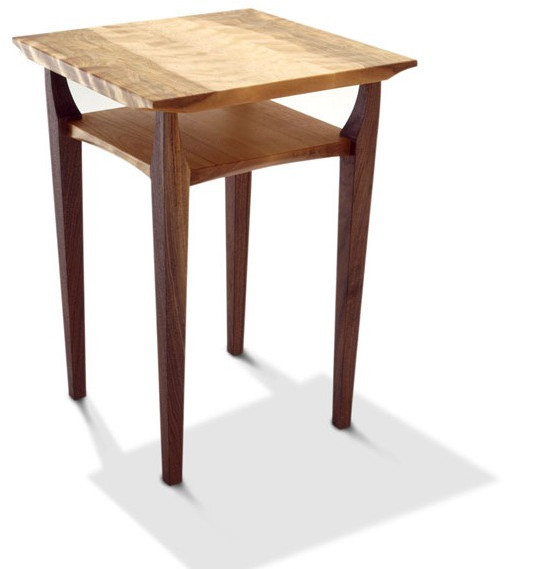
\includegraphics[width=0.4 \textwidth]{imgs/Aspiration-Nightstand-birch.jpg}
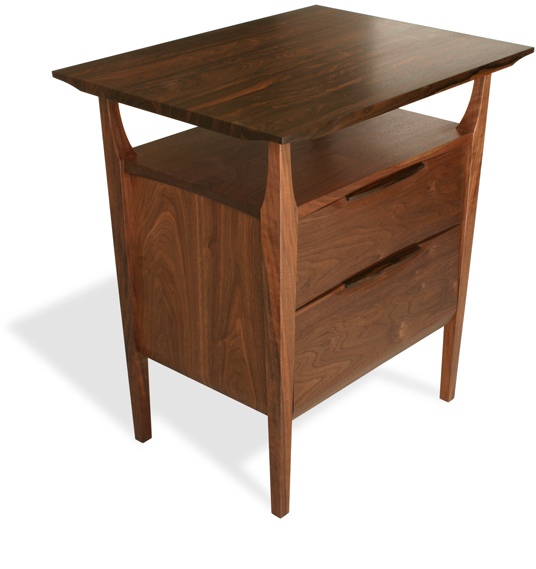
\includegraphics[width=0.4 \textwidth]{imgs/Aspiration-Nightstand-walnut.jpg}
}
\caption{Ende- og nat-bord fra \texttt{CITYJOINERY} i hhv. birk og valnød til
venstre, og valnød til højre.} \end{figure}

Projektet er et fribensmøbel med sarge, én skuffe hvis top fungerer som hylde,
og en bordplade. Projektet udføres i massiv valnød, med undtagelse af
skuffebund, hylde og bordplade, der alle laves af birke-krydsfiner med
valnøddefiner.
